\documentclass{tufte-handout}

%\geometry{showframe}% for debugging purposes -- displays the margins

\usepackage{amsmath}

% Set up the images/graphics package
\usepackage{graphicx}
\setkeys{Gin}{width=\linewidth,totalheight=\textheight,keepaspectratio}
\graphicspath{{graphics/}}

\title{Metabolic Control Systems}
\author{}
\date{}  % if the \date{} command is left out, the current date will be used

% The following package makes prettier tables.  We're all about the bling!
\usepackage{booktabs}

% The units package provides nice, non-stacked fractions and better spacing
% for units.
\usepackage{units}

% The fancyvrb package lets us customize the formatting of verbatim
% environments.  We use a slightly smaller font.
\usepackage{fancyvrb}
\fvset{fontsize=\normalsize}

% Small sections of multiple columns
\usepackage{multicol}

% Provides paragraphs of dummy text
\usepackage{lipsum}

% These commands are used to pretty-print LaTeX commands
\newcommand{\doccmd}[1]{\texttt{\textbackslash#1}}% command name -- adds backslash automatically
\newcommand{\docopt}[1]{\ensuremath{\langle}\textrm{\textit{#1}}\ensuremath{\rangle}}% optional command argument
\newcommand{\docarg}[1]{\textrm{\textit{#1}}}% (required) command argument
\newenvironment{docspec}{\begin{quote}\noindent}{\end{quote}}% command specification environment
\newcommand{\docenv}[1]{\textsf{#1}}% environment name
\newcommand{\docpkg}[1]{\texttt{#1}}% package name
\newcommand{\doccls}[1]{\texttt{#1}}% document class name
\newcommand{\docclsopt}[1]{\texttt{#1}}% document class option name

\begin{document}

\maketitle% this prints the handout title, author, and date

\begin{abstract}
\noindent This lecture will cover the basics of metabolic control, including how enzymes and transport systems control the fate of a metabolite and how systems are integrated to maintain homeostasis.
\end{abstract}

\tableofcontents

\pagebreak
\section{Learning Objectives}

\begin{itemize}
\item Understand what a rate limiting enzyme is, what a committed enzyme step is and what a reversible reaction is.
\item Explain the differences in speed and persistence of allosteric, post-translational and transcriptional regulation of metabolism.
\item Describe the role of cellular transport in macromolecular regulation. Understand the differences between active and passive transport.
\item Describe how hormones alter macronutrient metabolism after a meal.

\end{itemize}

\pagebreak

\section{Control of Metabolic Flux}

Cells need to control the rates at which nutrients are taken up, stored, or used and there are several ways by which this occurs.  We will review the biochemistry of both nutrient transport and enzyme function.  Understanding these concepts will be very important to understanding how the metabolic pathways we will discuss later in class are controlled. 

\section{Cellular Transport Systems}

First we will describe the ways in which cells control nutrient permability.  Most nutrients we will disscuss\sidenote{with the exception of sterols and some other lipids} are unable to pass through the plasma membrane of the cell.  Without these transport mechanisms we would be unable to absorb digested food, or transfer nutrients from cell to cell.  While we normally think of transporters as getting nutrients into or out of a cell, they are also important \emph{within} cells, for example getting pyruvate into the mitochondria, or storing calcium in the endoplasmic reticulum.

\subsection{Types of Membrane Transporters}

Membrane transporters are generally fairly specific for the macronutrient they transport.  For example GLUT4 transports glucose, but GLUT5 transports fructose.  Transporters can broadly be separated into two major types, passive transporters and active transporters.

\newthought{Passive transporters} allow for nutrients to pass down a concentration gradient into the cell.  For example, the liver expresses a glucose transporter named GLUT2.  Glucose can either enter the liver (if there is more glucose in the blood than the liver) or exit the liver (if the reverse is true).  Passive transporters will only allow a nutrient to enter a cell \emph{if there is less of the nutrient in a cell than in the blood}.  This is quite efficient for disposing of excess nutrients, such as after a meal, but is not effective in packing things away against a concentration gradient.  It may seem like passive transporters are not regulated, but as we will see in the case of GLUT4, the amount of transporters at the cell surface can be controlled by cell signaling (if you want to jump ahead, here is a review on that process \cite{Leto2012}).  The rate of a passive transport is defined by three things, the gradient of the tranported molecule, the number of transporters and the efficiency of the transporter.

\newthought{Active transporters} can force nutrients into a cell \emph{against} the concentration gradient.  These transporters function like pumps and have to use energy of one sort or another to "power" the molecule into the cell.  You may think that this is a bad idea, but there are lots of examples where this matters physiologically.  One example is retaining salt.  If your kidneys werent actively retaining sodim out of urine and back into the blood, then you would rapidly lose osmotic pressure in your blood.  \sidenote{We will discuss this example in detail in the lecture on electrolytes.}  The key is the think about the concentration inside or outside, if you are pushing against the transport gradient, you need active transport.

\subsection{Powering Active Transport}

Active transport requires energy of some type.  This energy can come from several sources such as ATP, other concentration gradients, or even light.  Some examples are described in Figure \ref{fig:active-transport-mechanisms} from Molecular Biology of the Cell\cite{Alberts2002a}.  The key to controlling the rate of these transporters is not only the concentration gradient of the transported molecule, but also the levels (or gradient) of the powering force.  In the cases where molecules are co-transported they can either be pulled in simultaneously (this is known as a symporter) with the molecule of interest as shown on the left of Figure \ref{fig:active-transport-mechanisms}, or can be exchanged where one molecule exits, powering the entry of the molecule of interest (this is known as an antiporter).  A classic example of an antiporter is the sodium:glucose exchanger SGLT1, which extrudes sodium down its concentration gradient (into the gut lumen) to force uptake of glucose from the gut into cells.  This allows for efficient carbohydrate uptake in a meal\sidenote{SGLT2 does a similar thing, retrieving glucose from urine back in to the blood, and is the target of several drugs which try to lower blood glucose in diabetics by blocking this process.  The trade names for these drugs include Invokana, Farxiga and Jardiance.}

\begin{marginfigure}
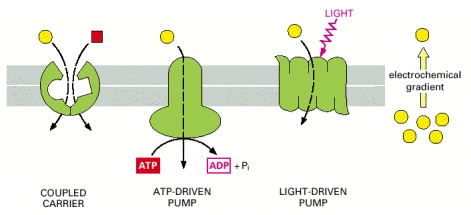
\includegraphics{figures/active-transport-mechanisms.jpg}\
\caption{Examples of active transport.}
\label{fig:active-transport-mechanisms}
\end{marginfigure}

\section{Enzymes}

\subsection{Thermodynamics}

\newthought{Every chemical in the body has a certain amount of energy.}  When we eat, some of this chemical energy is converted into ATP to allow for function.  This is known as catabolism.  When we are storing nutrients, we use ATP to generate higher energy molecules such as fats or glycogen.  This is known as anabolism.  Every molecule in our body has a set amount of energy a chemical reaction can be considered endothermic (requiring energy) or exothermic (releasing energy), depending on whether the reactants or products have higher energy.  The levels of these metabolites at equillibrium can be calculated with the following equation where K$_{eq}$ is the \emph{Eqiullibrium constant}\sidenote{brackets mean the concentration of A or B}:

\begin{equation}
[A]=K_{eq}[B]
\end{equation}

 The equillibrium constant can be calculated from the \emph{free energy} of the reactants and products.

\begin{equation}
\Delta G_{o} = G^{'}_{o} - R T ln K_{eq}
\end{equation}
\begin{equation}
\Delta G^{'}_{o} = G^{'}_{o} (reactants) - G^{'}_{o} (products) 
 \end{equation}


Some reactions have products with very similar energy levels and the balance between the reactants and the products is based only on their concentrations.  This is known as an \emph{equillibrium} reaction which would have a K$_{eq}$ of near to 1.  If a reaction requires a lot of energy to occur, this is often an \emph{irreversible} or \emph{committed} step\sidenote{This would have a large, negative K$_{eq}$}.  This means that once this reaction happens, there is no going back.  If you think about the metabolic pathway in Figure \ref{fig:committed-step}, this would mean that once you proceed through step 2 to make  C you cannot go back to B.  Therefore given the free energy and concentration of the reactants and products in a reaction you can calculate the $\Delta G$ and equillibrium constant for a reaction and estimate whether it is reversible.\sidenote{There is a good blog post explaining how the steady state $\Delta G$ is determined on this basis at \url{http://sandwalk.blogspot.com/2007/10/aldolase-reaction-and-steady-state.html}}

\begin{marginfigure}
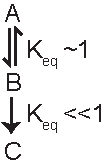
\includegraphics[width=0.5\marginparwidth]{figures/committed-step.pdf}\
\caption{Example schematic of a metabolic pathway.}
\label{fig:committed-step}
\end{marginfigure}

\subsection{Enzyme Kinetics}

\newthought{In terms of how fast a reaction occurs,} rather than the levels at equillibrium, in the body most reactions are normally very slow without enzymes.  Enzymes function to increase the rate of a chemical reaction.  They do this by reducing the activation energy required for a reaction to occur, but does not change the equillibrium constant.  This is described in Figure \ref{fig:enzymatic-rates}, note that $\Delta G$ is not changed, but the dashed line has a higher activation energy, and therefore slower reaction rate than the solid line.  

\begin{marginfigure}
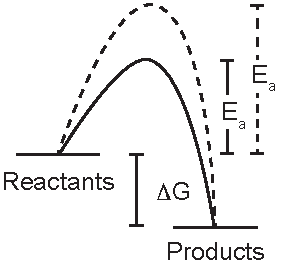
\includegraphics[width=\marginparwidth]{figures/enzymatic-rates.pdf}\
\caption{Example schematic of the activation energy (E$_a$) of an enzymatic reaction.}
\label{fig:enzymatic-rates}
\end{marginfigure}

\newthought{Most metabolic pathways are controlled by altering the rates} at which metabolites are converted to its final product. The overall rate of a metabolic pathway is controlled by the \emph{rate-limiting step}\sidenote{the rate-limiting step is generally the \emph{slowest} step of a pathway.  As an example, in glycolysis the rate-limiting step is catalysed by phosphofructokinase-1}.  In a linear pathway, the speed of this step's enzymatic reaction controls the overall rate.  Quite often this enzyme is an important site of regulation, as adjusting the speed of this reaction can speed up or slow down and entire pathway.  Reaction rates increase in rate as the amount of substrates increase until the enzymes are saturated (see the solid line in Figure \ref{fig:enzyme-kinetics}).  This is known as Michaelis-Menten kinetics.  The reaction rate constant (k) and rate can be calculated from the activation energy with these equations\sidenote{A and R are constants, T is temperature and e is Euler's number.  $K_{m}$ is the Michaelis constant for an enzyme.}:

\begin{equation}
k = A e^{-\frac{E_{a}}{RT}} 
\end{equation}
\begin{equation}
rate = k\tfrac{[Reactant][Enzyme]}{[Reactant] + K_{m}}
\end{equation}

If products build up the reaction becomes more complex and now looks like this where K$_{p}$ is the binding constant for the product:

\begin{equation}
rate = k\tfrac{[Reactant][Enzyme]}{[Reactant] +K_{m}\left \{ 1 + \frac{[Product]}{Kp} \right \}}
\end{equation}

\begin{marginfigure}
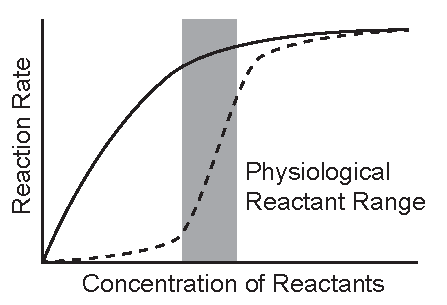
\includegraphics[width=\marginparwidth]{figures/enzyme-kinetics.pdf}\
\caption{Example of Michaelis-Menten (solid line) and allosteric (dashed line) kinetics.}
\label{fig:enzyme-kinetics}
\end{marginfigure}

\newthought{Allosteric regulation is another way by which enzymes can control reaction rates}.  Allosteric enzymes are generally multi-subunit enzymes that change their K${m}$ as more products bind.  An example of this is the dashed line in Figure \ref{fig:enzyme-kinetics}.  This has several advantages in terms of regulation.  One advantage is that the reaction rate can be effectively zero or at maximum in a much narrower range, bracketing the actual range of substrates present physiologically.  Another advantage is that allosteric activators or inhibitors can shift the curve to the left or right, to effectively increase or decrease the reaction rate. 

On the basis of these equations, reaction rates and therefore the efficiency of a particular pathway can be increased by several things\sidenote{Some examples include:\\\begin{enumerate}
\item Decreasing the activation energy
\item Increase the amount of the substrate(s)
\item Decrease the amount of the product(s)
\item Increase the number of enzymes
\item Decreasing the K$_m$ of the enzyme
\item Shifting the substrate sensitivity of the allosteric enzyme
\end{enumerate}	}.  Try to convince yourselves how this happens based on the equations listed above. Can you think of any other things that would affect pathway flux? 

\newthought{While linear flow through a pathway is important}, another aspect of pathway control is how the fate of a particular nutrient is decided.  This is illustrated in Figure \ref{fig:nutrient-pathways}.  In the example on top the nutrient would be equally distributed between three products, but in the bottom example, by adjusting the rates of the specific pathways, a nutrient can be directed to a particular product.  

\begin{marginfigure}
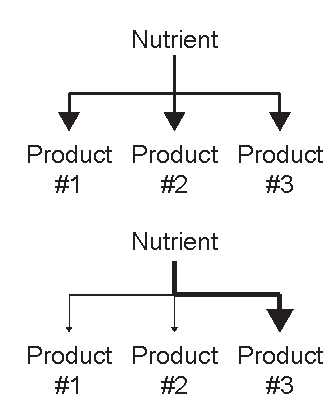
\includegraphics[width=0.75\marginparwidth]{figures/nutrient-pathways.pdf}\
\caption{Example of how regulated pathways control nutrient fate.}
\label{fig:nutrient-pathways}
\end{marginfigure}

\section{Integrated Control of Metabolism}

There are several ways in which enzymes are regulated, both based on intracellular and extracellular signals.  An example might be that a lack of intracellular ATP causes an increase in ATP producing pathways such as glycolysis.  On the other hand, low circulating blood glucose levels may work to stop a glucose consuming process such as that.  We will discuss this in detail throughout the lecture, but some of the hormones we will discuss in this course that are particularly important are listed in Table \ref{tab:hormones}:

\begin{table}[h]
\centering
\caption{Some important metabolic hormones we will discuss in this class.}
\label{tab:hormones}
\begin{tabular}{cc}
\hline
\textbf{Hormone}       & \textbf{Main Function}                     \\
\hline
Insulin                & Reduces blood glucose and lipid levels     \\
Adrenaline			   & Increases blood flow, nutrients to muscle \\
Glucagon               & Increases blood glucose levels acutely     \\
Cortisol               & Increases blood glucose levels chronically \\
GH/IGF1                & Promotes protein synthesis and bone growth \\
Testosterone           & Promotes protein synthesis                 \\
Leptin                 & Suppresses appetite                        \\
CCK, Gastrin, Secretin & Regulation of digestion                   \\
\hline
\end{tabular}
\end{table}


Hopefully these hormones, how they work and how they are regulated is material you are familiar with from previous classes.  If not, or you want a refresher, check out the \textbf{Endocrine Control of Macronutrient Metabolism} handout also available on Canvas.  

\newthought{For more detailed overview of these fundamental basics of biochemistry}, two textbooks are on reserve at the Shapiro library for this course \cite{Berg2013} and \cite{Ferrier2017} and are available free online (\textit{e.g.} \url{https://www.ncbi.nlm.nih.gov/books/NBK21154})

\bibliography{library}
\bibliographystyle{plainnat}

\end{document}
